\ifthenelse{\orcert=1}{

\begin{figure}[ht]
    \setlength{\parindent}{-10pt}
    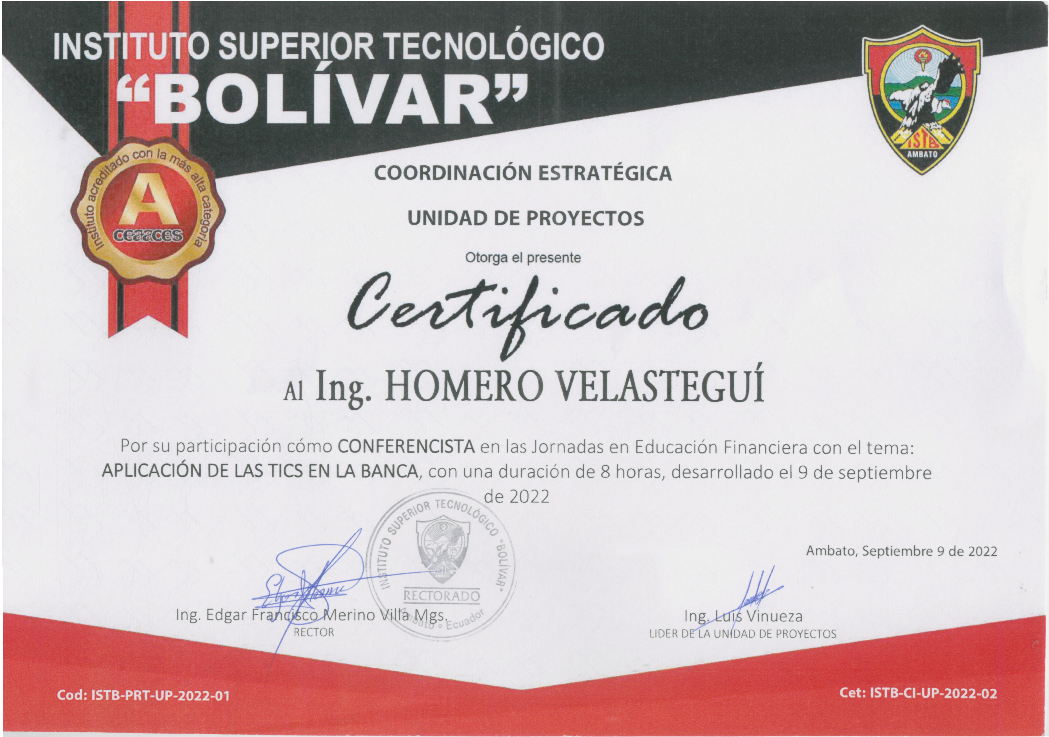
\includegraphics[width=0.95\textwidth]{3.-Ponencias/Certificados/4.png}
\end{figure}


\begin{figure}[ht]
    \setlength{\parindent}{-10pt}
    \href{https://n9.cl/h5qad}{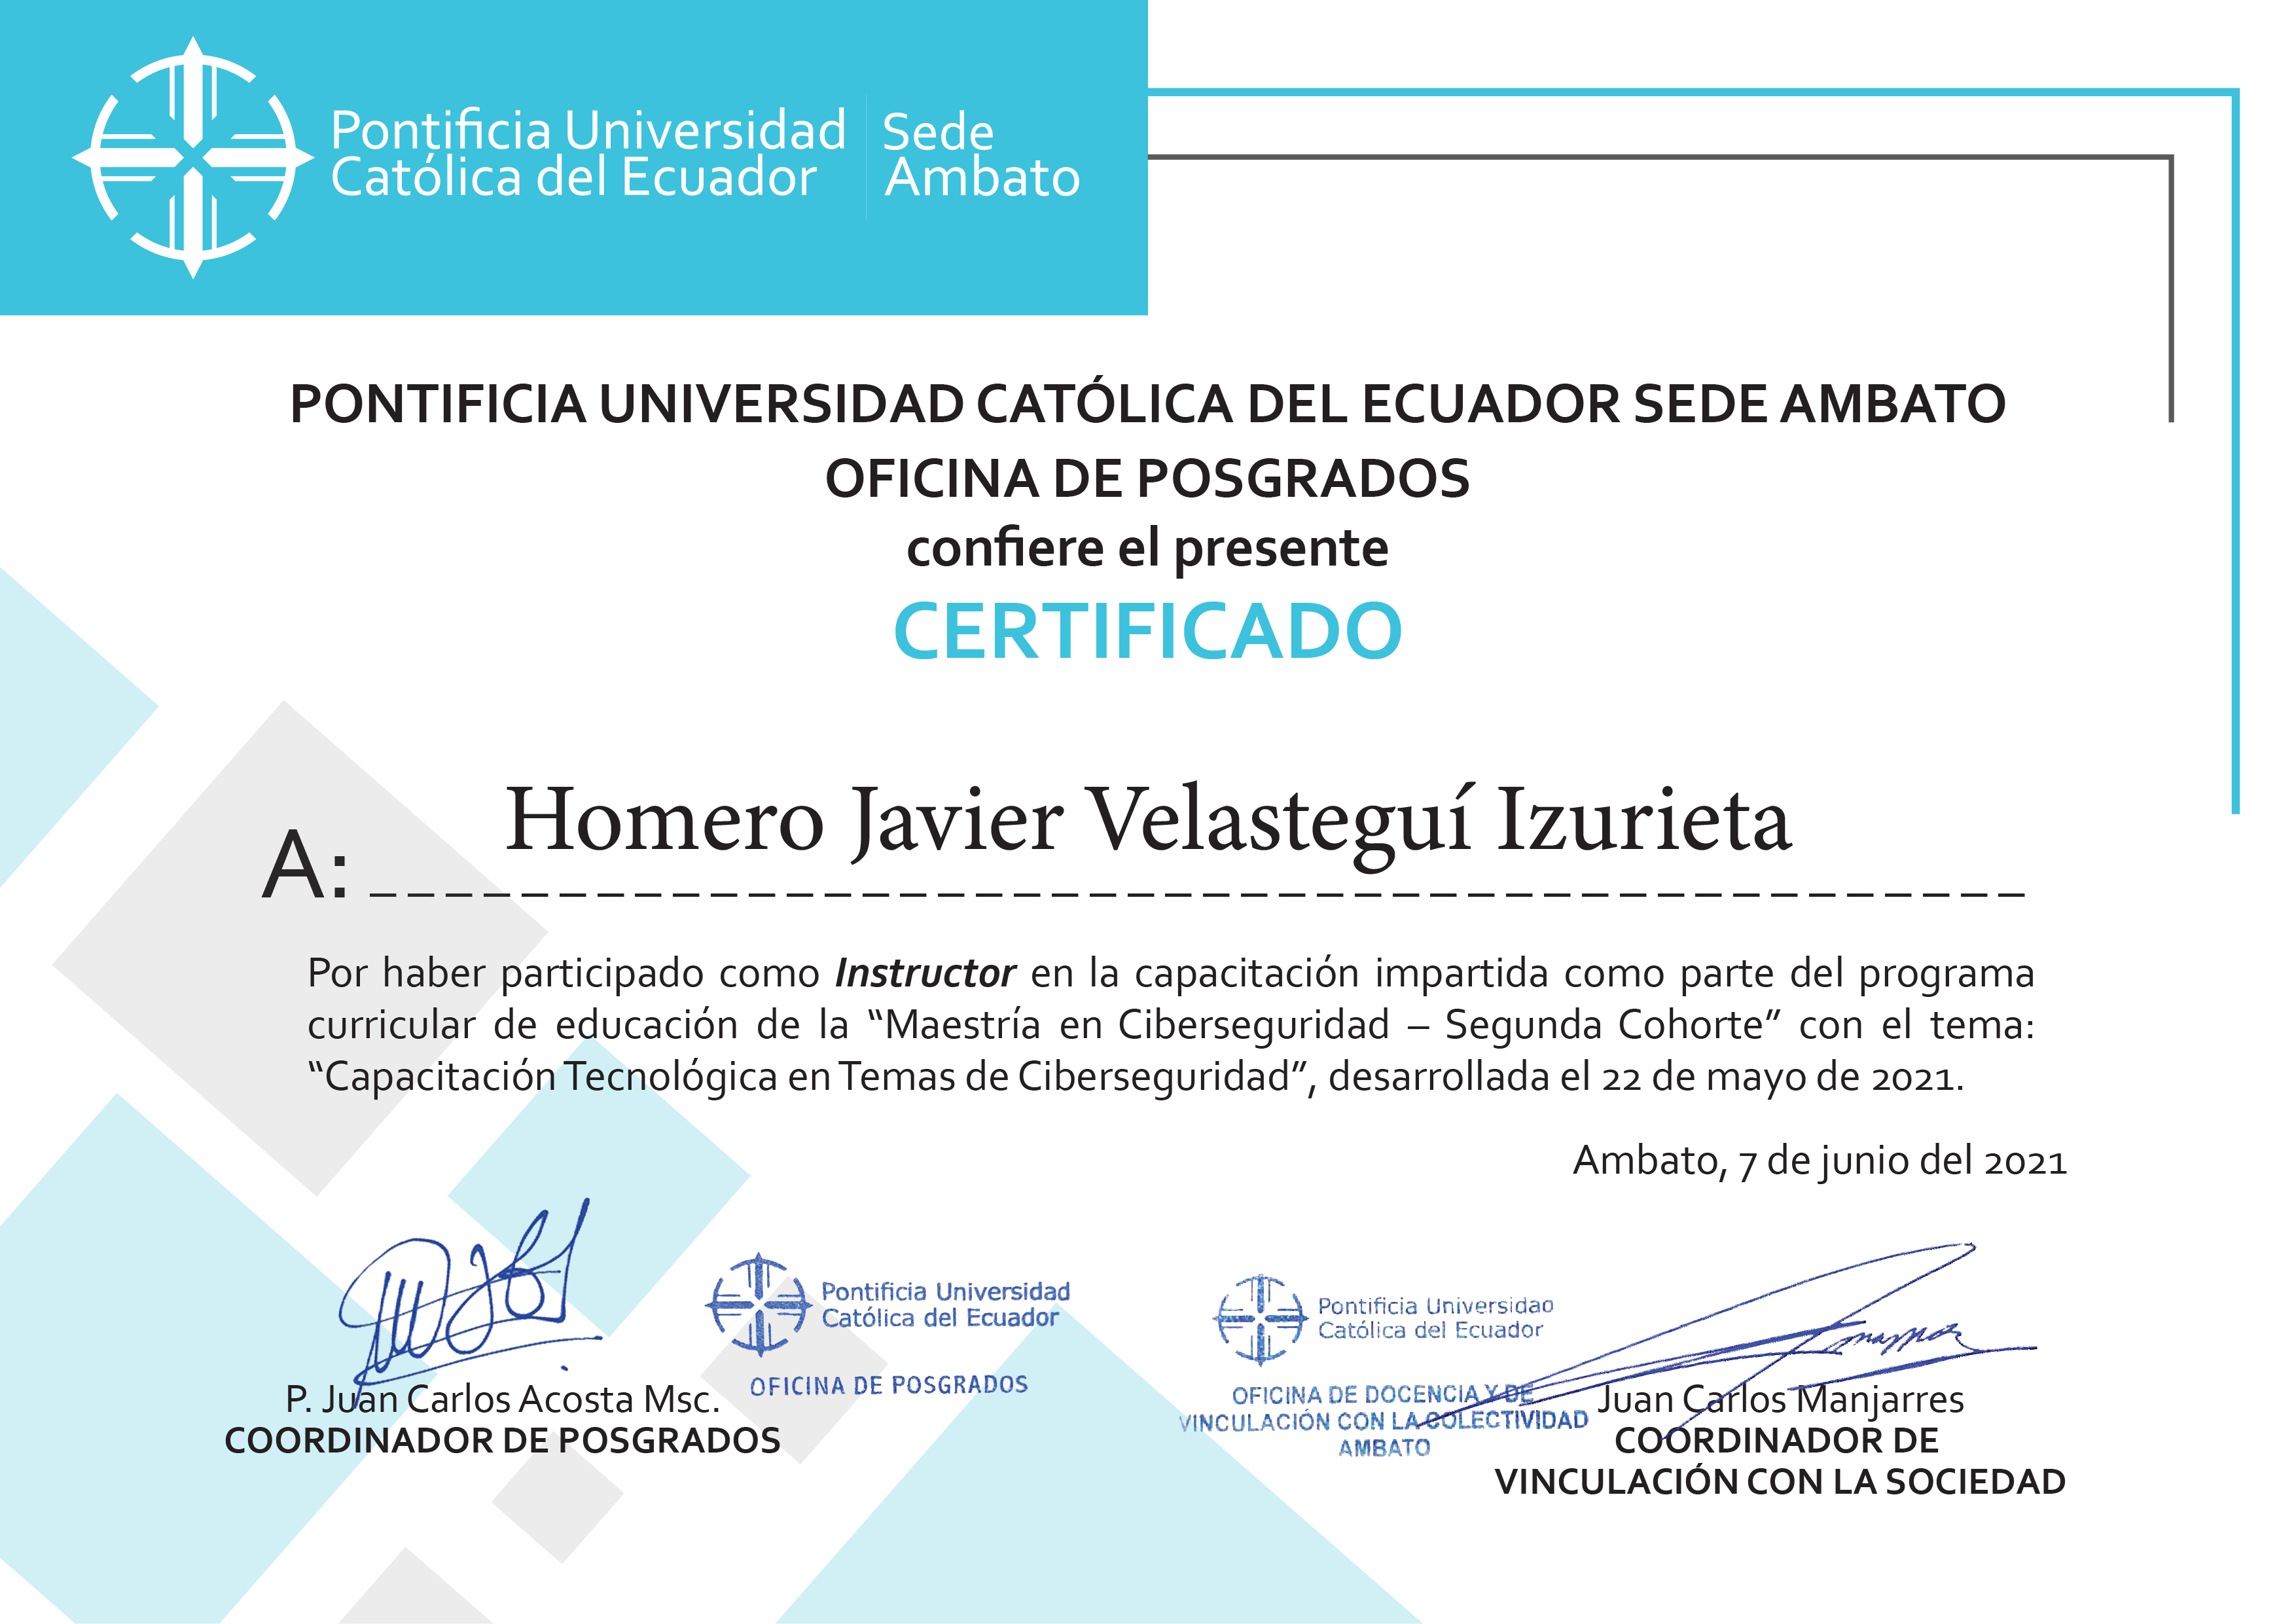
\includegraphics[width=0.95\textwidth]{3.-Ponencias/Certificados/3.jpg}}
\end{figure}

\begin{figure}[ht]
    \setlength{\parindent}{-10pt}
    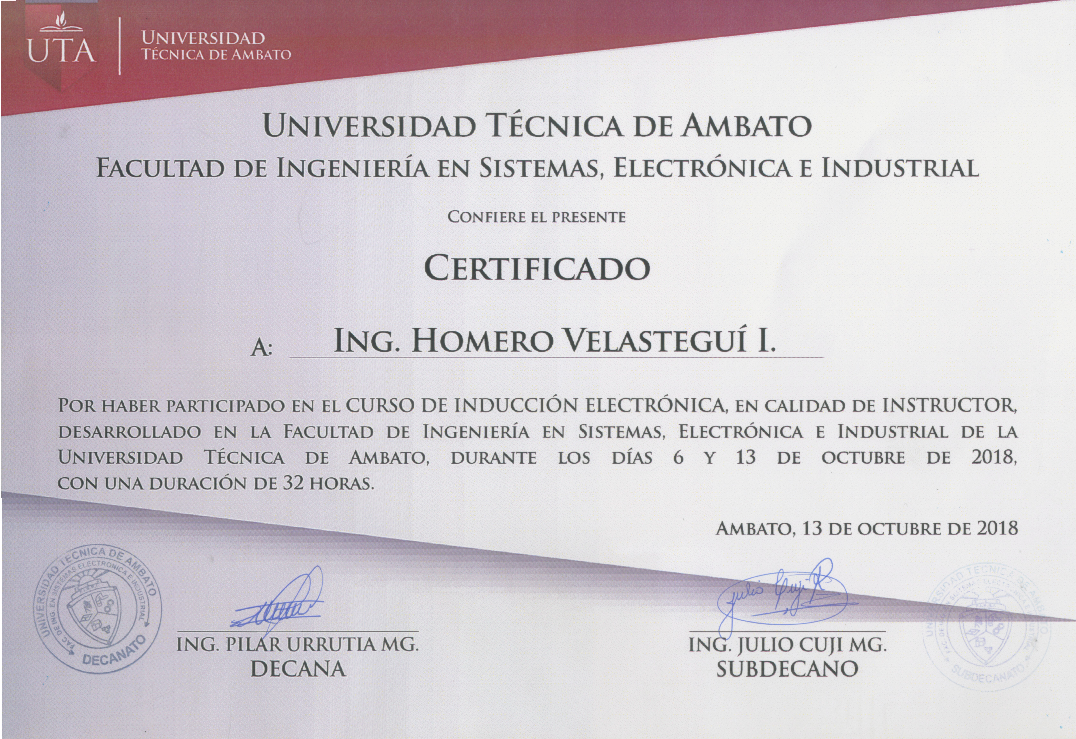
\includegraphics[width=0.95\textwidth]{3.-Ponencias/Certificados/2.png}
\end{figure}




\begin{figure}[ht]
    \setlength{\parindent}{-10pt}
    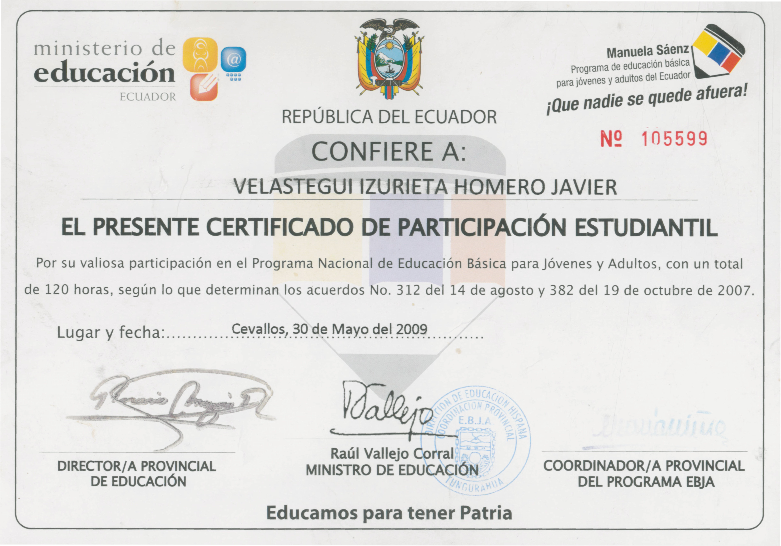
\includegraphics[width=0.95\textwidth]{3.-Ponencias/Certificados/1.png}
\end{figure}
}{
\begin{figure}[ht]
    \setlength{\parindent}{-20pt}
    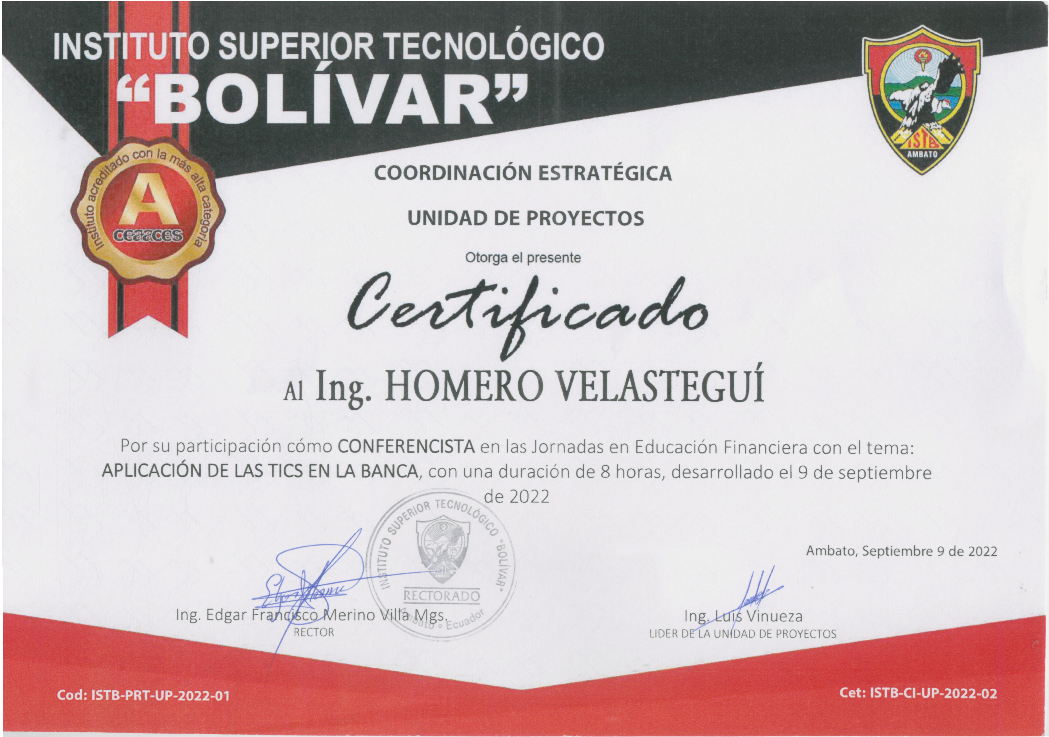
\includegraphics[width=1.4\textwidth, angle=90]{3.-Ponencias/Certificados/4.png}
    \centering
\end{figure}

\begin{figure}[ht]
    \setlength{\parindent}{-20pt}
    \href{https://n9.cl/h5qad}{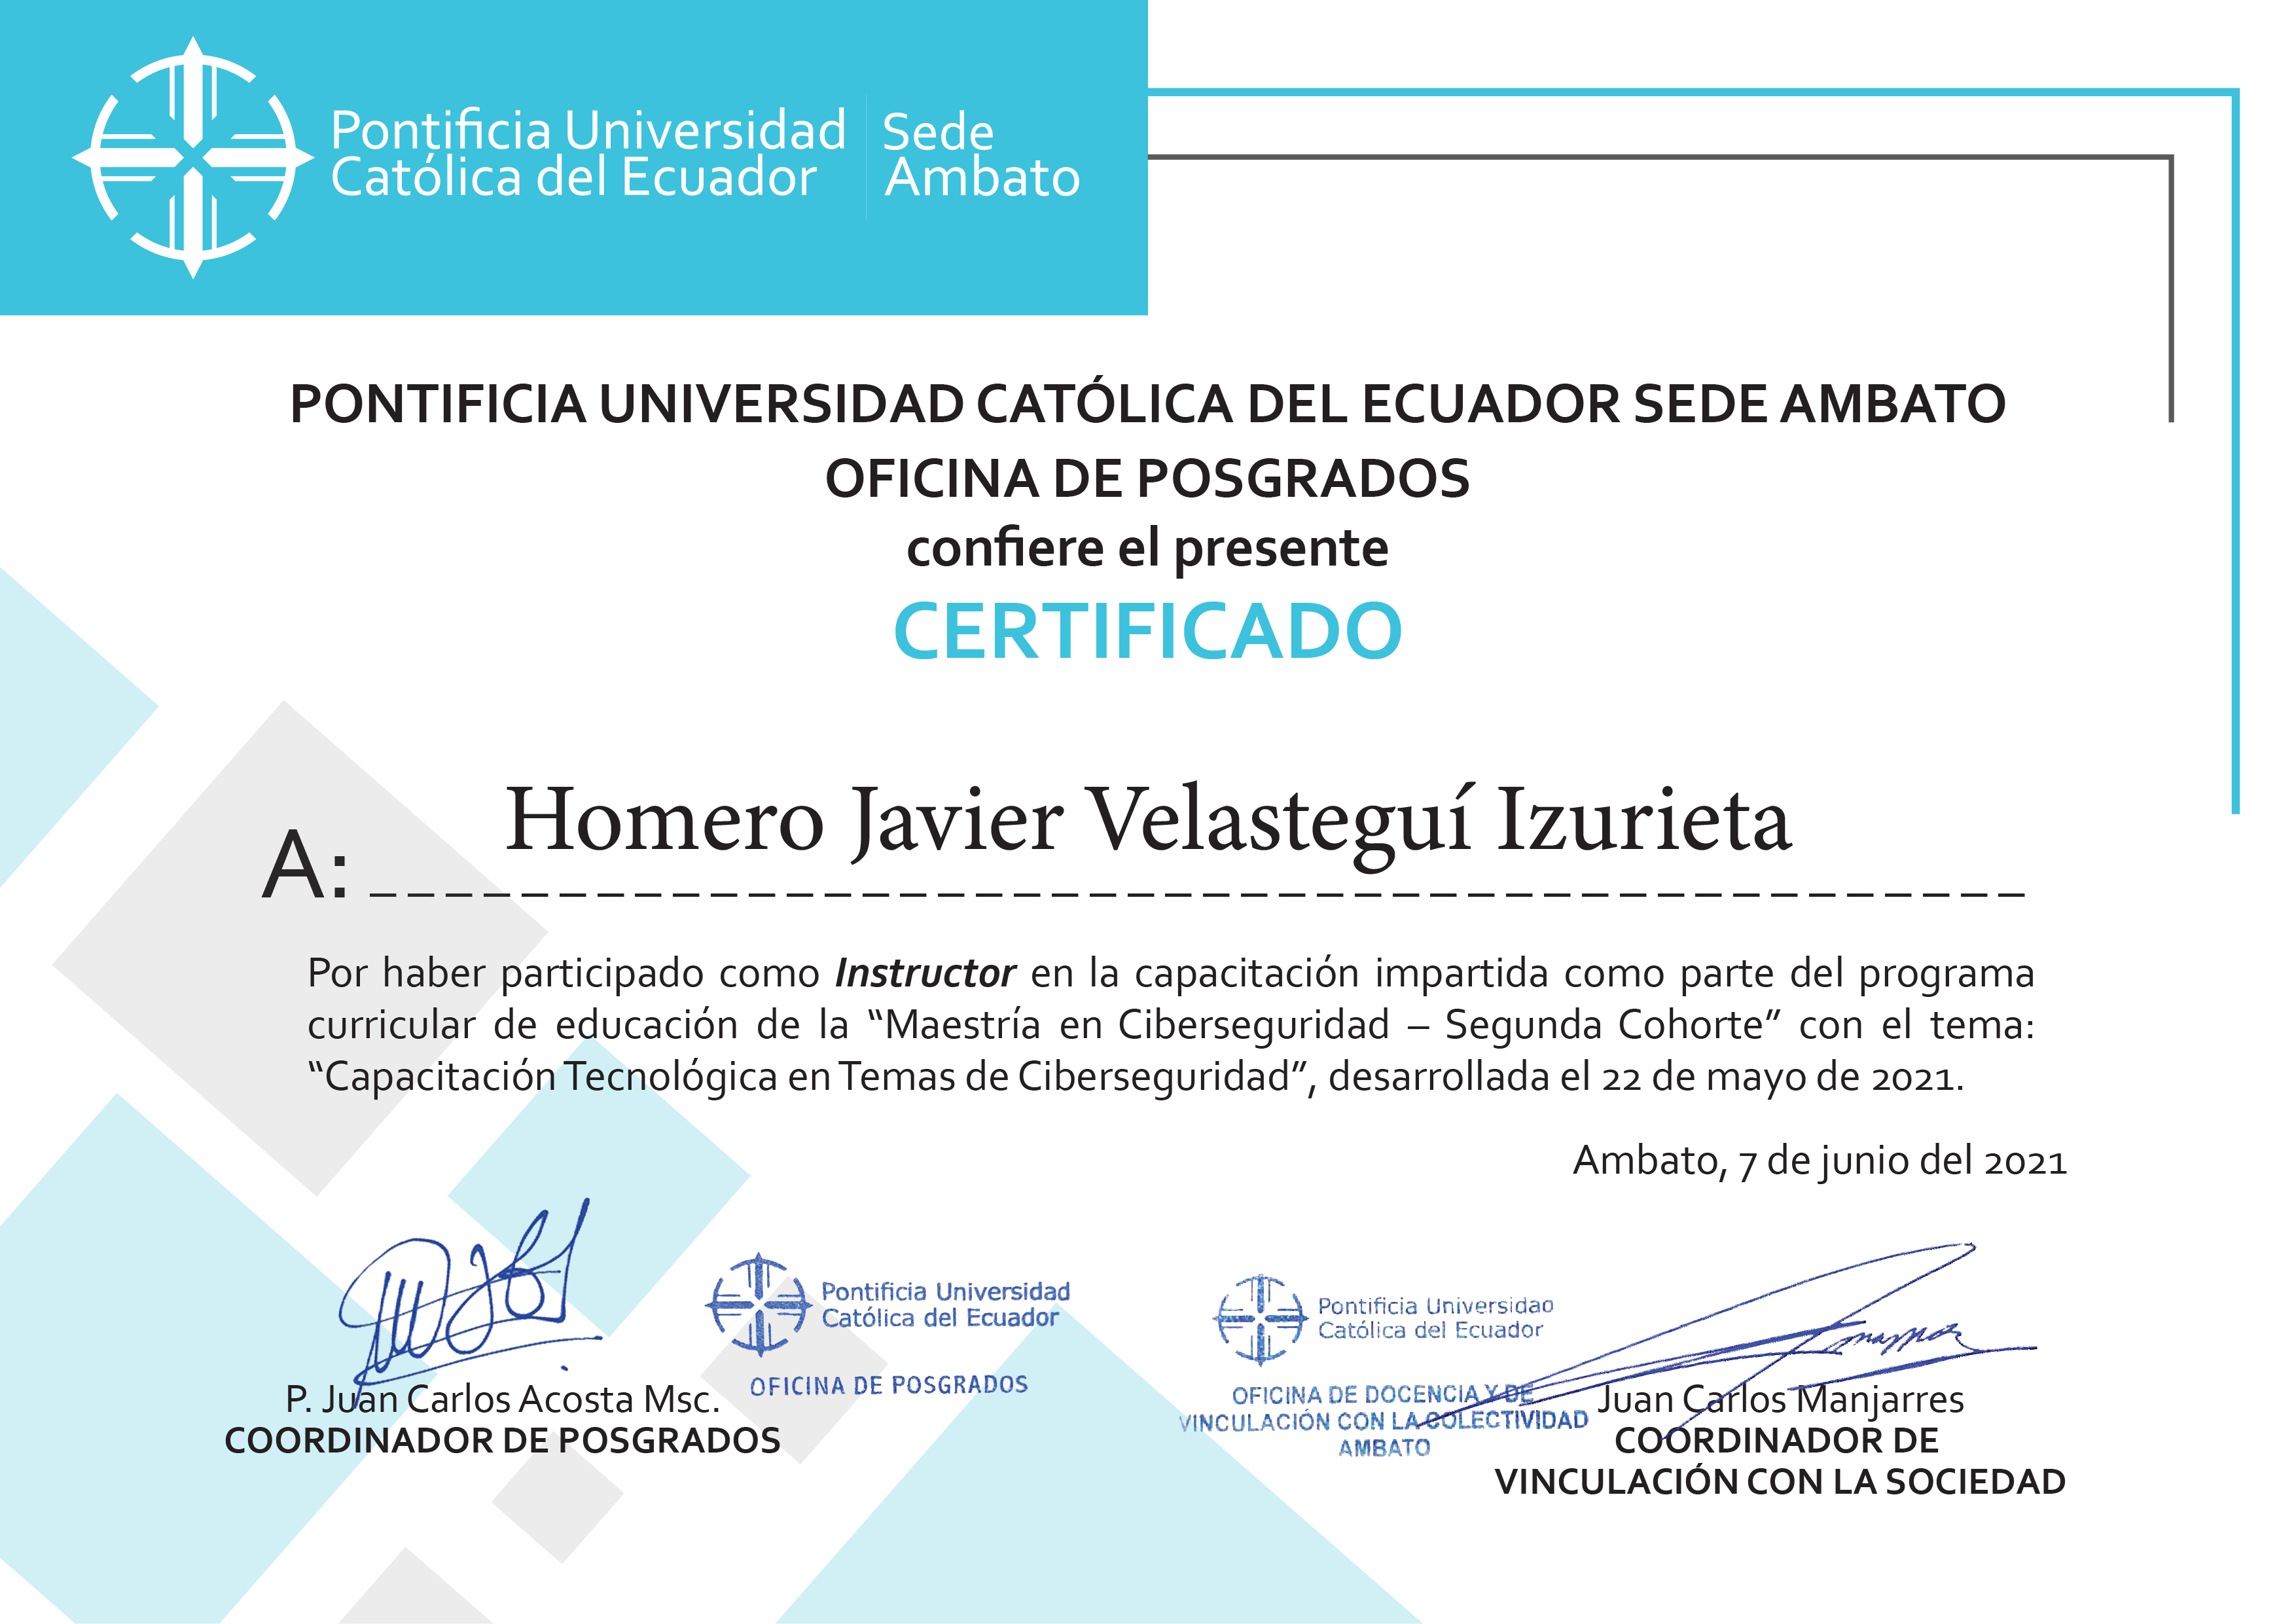
\includegraphics[width=1.4\textwidth, angle=90]{3.-Ponencias/Certificados/3.jpg}}
    \centering
\end{figure}

\begin{figure}[ht]
    \setlength{\parindent}{-10pt}
    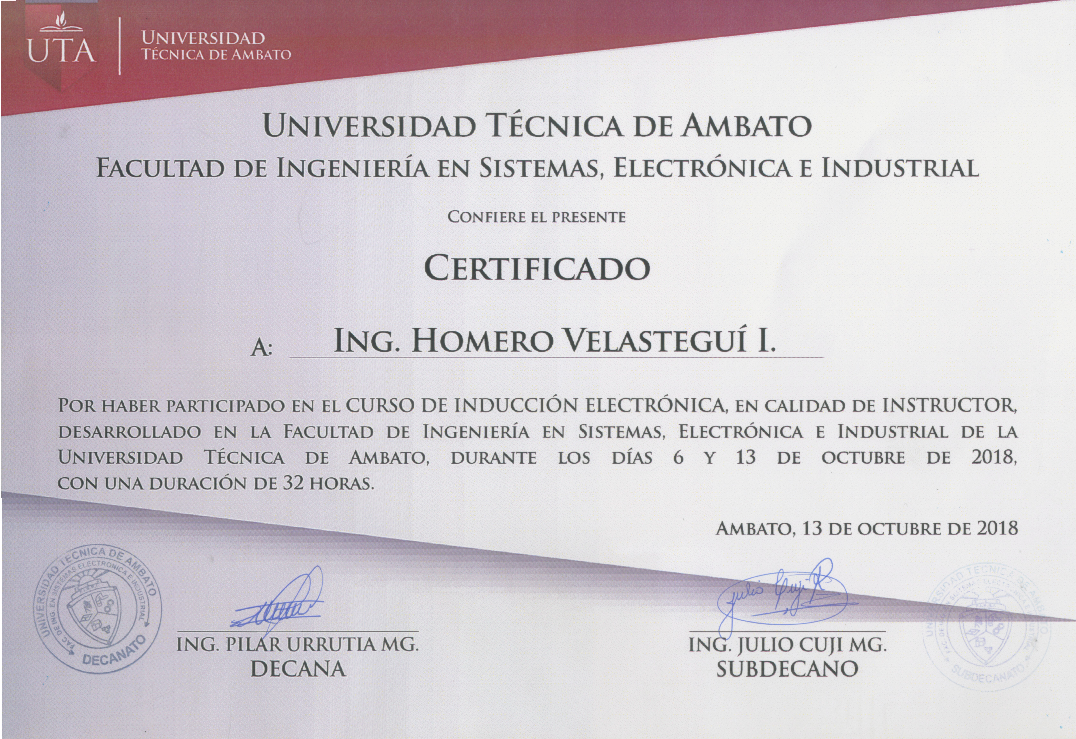
\includegraphics[width=1.4\textwidth, angle=90]{3.-Ponencias/Certificados/2.png}
    \centering
\end{figure}



\begin{figure}[ht]
    \setlength{\parindent}{-10pt}
    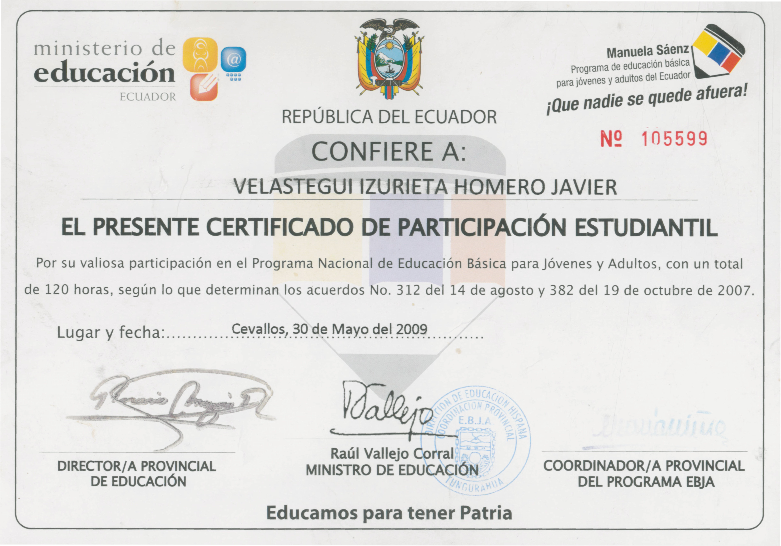
\includegraphics[width=1.4\textwidth, angle=90]{3.-Ponencias/Certificados/1.png}
    \centering
\end{figure}

}